\documentclass[12pt]{article}

\usepackage[a4paper, left=2.5cm, right=2.5cm, top=2.5cm, bottom=2.5cm]{geometry}
\usepackage{times}

\usepackage[utf8]{inputenc}
\DeclareUnicodeCharacter{2212}{$-$} % Minus sign
\DeclareUnicodeCharacter{03BC}{µ}

\usepackage[british]{babel}
\usepackage{csquotes}

\usepackage[font=small, labelfont=bf]{caption}
\usepackage[labelformat=parens, labelfont=bf, subrefformat=parens]{subcaption}

\usepackage[indent=0pt]{parskip}
\usepackage{setspace}
\onehalfspacing

\usepackage{graphics,graphicx}
\usepackage{svg}
\graphicspath{{../Figures/}}
\usepackage{float}

% Maths formatting
\usepackage{amsmath}
\usepackage{braket}

% Clever references
\usepackage[hidelinks]{hyperref}
\urlstyle{same}
\usepackage[nameinlink,capitalise,noabbrev]{cleveref}
\crefname{condition}{Condition}{Conditions}

\usepackage{amsthm}
\newtheorem*{theorem}{Theorem}
\theoremstyle{definition}
\newtheorem*{definition}{Definition}
\newtheorem{condition}{Condition}

% Bibliography
\usepackage[style=trad-abbrv, maxnames=2, date=year, backend=biber, sorting=none]{biblatex}
\addbibresource{thesis.bib}

\usepackage{xurl}

% Number formatting
\usepackage[mode=text]{siunitx}
\sisetup{
    round-mode=figures, round-precision=3, round-pad=false,
    range-phrase=--, range-units=single
}

%\usepackage{multirow} % Multi-row cells in tables
%\usepackage{booktabs} % Nice table separators

\title{\Huge \bfseries Quantum annealing\\for music arrangement}
\author{Lucas Kirby\\\normalsize Department of Physics, University of Durham\\\\\normalsize Supervised by\\\normalsize Prof Robert Potvliege \& Dr Omer Rathore}
\date{\normalsize 23 April 2025}

\begin{document}

\maketitle

\vfill

\addcontentsline{toc}{section}{Abstract}
\begin{abstract}              

Music arrangement is usually a complex and time-consuming process; this paper aims to provide an automatic method by which to arrange music via a quantum computing technique called quantum annealing. By splitting a score into a set of phrases, these phrases can form a quadratic unconstrained binary optimisation (QUBO), a function which the quantum computer aims to minimise by choosing the values of discrete variables. At the end of the optimisation process, the resulting chosen values describe the final arrangement, which can then be interpreted into sheet music.

\end{abstract}

\vfill

\begin{center}
    \includesvg{durham-university.svg}
\end{center}

\thispagestyle{empty}
\clearpage

\tableofcontents
%\listoffigures

\thispagestyle{empty}
\clearpage

\section{Introduction}

% Background to quantum computing
The field of quantum computing has its foundations as early as the 1980s, with the suggestion that hardware following the laws of quantum mechanics could be faster and more powerful than its classical counterpart \cite{feynman_simulating_1982}.
Quantum computers, which leverage quantum mechanical phenomena to perform calculations, store information as qubits (``quantum bits'') which can exploit effects such as superposition and entanglement to increase computing power.
As quantum computers developed, along with them came the possibility to solve complex problems usually intractable to even the most powerful classical computers, an advantage dubbed ``quantum supremacy'' \cite{preskill_supremacy_2012}. This is not to say that quantum computers can solve problems that are impossible for classical computers, but that they can solve them faster. A collaboration between Google AI Quantum and NASA became the first to claim quantum supremacy in 2019 \cite{arute_quantum_2019}, although this claim has since been refuted \cites{pednault_leveraging_2019}{mccormick_race_2022}. More recently, D-Wave Quantum Systems Inc.\ claimed to have demonstrated quantum supremacy simulating quantum critical dynamics, performing magnetic materials simulations in minutes that would take nearly one million years using classical supercomputers \cite{king_beyond_2025}. However, this claim too was quickly challenged \cites{tindall_dynamics_2025}{mauron_challenging_2025}. Skepticism about quantum computers has existed since their conception \cite{unruh_maintaining_1995} and is still ongoing \cite{brooks_quantum_2023}, but this does not prevent many from being optimistic about future applications.

Since its inception, two methods of quantum computing have been developed: gate-based computing and adiabatic quantum computing.
% Gate-based
Gate-based quantum computers use quantum gates to manipulate qubits, analogous to classical logic gates for conventional circuits, where gates can be represented as operators acting on qubit states. This kind of computer is versatile and well-suited to solving general problems, and is being actively developed by several technology companies as the next step in general computing \cites{google}{ibm}.
% Quantum annealing
Adiabatic quantum computers, on the other hand, rely on the application of the adiabatic theorem to slowly evolve a quantum system. This is often used to find the global minimum of a given function which would be almost impossible to solve analytically. Adiabatic quantum computers have been used to find solutions to a variety of optimisation problems, such as protein folding \cite{perdomo-ortiz_protein_2012}, financial portfolios \cite{phillipson_portfolio_2021}, and traffic flow \cite{inoue_traffic_2021}, although only within the limits of classical optimisation algorithms.

% Computer music
The combination of computing and music is a relatively new field, with the involvement of quantum computers even more so. Music is often seen as a very human endeavour, where only skilled musicians could compose and perform such sequences of sound that would be considered art. The idea that computers could produce music arose as early as the 19th century, with the conception of the first general-purpose computer, the Analytical Engine\footnote{The computer was never actually built, but laid the foundation for many modern computing concepts.}. It was noted that, given ``the fundamental relations of pitched sounds in the science of harmony and of musical composition\dots the engine might compose elaborate and scientific pieces of music of any degree of complexity or extent'' \cite{lovelace_sketch_1843}. The first computer composition would not be produced until nearly a century later \cite{hiller_experimental_1959}, and since then various classical approaches to computer music have been taken, including Markov chains, evolutionary models, and neural networks \cite{wiggins_composition_1999}. Quantum computing is the latest iteration of computer music, opening up new and unique possibilities.

% Quantum computer music
Since its emergence into the computer music scene, quantum computers have been used to write melodies \cite{miranda_teaching_2022}, develop harmonies \cite{arya_music_2022}, create vocal synthesisers \cite{miranda_quantum_2020}, and create intelligent musical systems via quantum natural language processing (QNLP) \cite{miranda_quantum_2021}, using a mixture of gate-based and adiabatic methods. It is emphasised that, whilst these techniques could just as well be implemented on classical computers, the motivation is ``the music technology community should be quantum-ready for when quantum computing hardware becomes more sophisticated'' \cite{miranda_quantum_2020}. However, all these efforts have been directed at music \emph{composition}, that is, the generation of entirely new sequences and sounds, rather than music \emph{arrangement}, the adaptation of previously-composed pieces. Indeed, at time of writing, the application of quantum computing to the problem of music arrangement has never been explored before.

% Study overview
In this study, we propose that music arrangement can be formulated as an optimisation problem to be solved using a heuristic application of adiabatic quantum computing called quantum annealing.
The structure of the study is as follows: we first introduce the relevant theory for both quantum annealing as a computational tool, and music arrangement as a suitable problem to solve; we then propose an original framework for combining the two, and apply this method to two musical scores; finally, we consider conclusions and possible future work.

\section{Quantum annealing}

As mentioned, quantum annealing falls under the category of adiabatic quantum computing (AQC). AQC is a computing technique that relies on the adiabatic theorem \cite{born_beweis_1928}.

\begin{theorem}[Adiabatic theorem]
    A physical system remains in its instantaneous eigenstate if a given perturbation is acting on it slowly enough and if there is a gap between the eigenvalue and the rest of the Hamiltonian's spectrum.
    \label{thm:adiabatic}
\end{theorem}

A linear evolution of the Hamiltonian of a system can be expressed as
\begin{equation}
    H(t)=\left(1- \frac{t}{T}\right)H_0 + \frac{t}{T}H_p
    \label{eq:time-evolution}
\end{equation}
where the system is evolving from an initial Hamiltonian $H_0$ to a final Hamiltonian $H_p$ over a time interval $T$. According to the adiabatic theorem, if the system starts in the $n$th eigenstate of $H_0$, then, given that the evolution is slow enough and that there is some energy difference between eigenstates (i.e.\ non-degeneracy), it will remain in the $n$th instantaneous eigenstate of $H(t)$ throughout evolution and end in the $n$th state of $H_p$. How ``slow'' the evolution needs to be is determined by the minimum energy gap of the instantaneous Hamiltonians; an approximate adiabaticity criterion can be given by
\begin{equation}
    \frac{\hbar\braket{\psi_m|\dot{H}|\psi_n}}{(E_n-E_m)^2} \ll 1
    \label{eq:energy-gap}
\end{equation}
where we have used the largest matrix element between a pair of adjacent eigenstates $\psi_{n,m}$, and ${E_n-E_m}$ is the minimum energy gap \cite{sakurai_quantum_2020}. It can be seen that a smaller energy gap requires a slower evolution in order to remain adiabatic, and that for degenerate energies ($\Delta E=0$) no adiabatic evolution is possible. 

This technique is useful as it allows particular eigenstates (usually the ground state) of a very complicated Hamiltonian ($H_p$) to be found simply by evolving from a Hamiltonian whose eigenstate is easy to find and prepare ($H_0$) \cite{farhi_quantum_2001}. Importantly, this process is universal and deterministic---if the system starts in the ground state of $H_0$, then it is guaranteed to be in the ground state of $H_p$ after adiabatic evolution.

However, since a truly adiabatic process takes infinitely many steps and therefore an infinite amount of time, this is not possible in practice. Instead, the adiabaticity condition of AQC can be relaxed to allow a shortening of the evolution time---this is quantum annealing\footnote{In metallurgical terms, annealing is the process of heating and cooling a material to alter its physical properties. Much like its metallurgical counterpart, quantum annealing allows a system to settle into a more useful final state.}. Over these shortened timescales ($T\sim\unit{\us}$), the process is now heuristic and the eigenstate after evolution is no longer guaranteed. The criterion given by \cref{eq:energy-gap} is not met and there is a possibility that the system is excited to a higher-energy state. The advantage of this method is that a particular evolution can be run many times, sampling the distribution of final states until an acceptable outcome is found.

Quantum annealing is used to solve combinatorial optimisation problems, which are problems that require the minimisation of a function over a discrete set of variables. If $H_p$ is defined such that its ground state encodes the most optimal solution to such a problem, then as long as the system is prepared in the ground state of $H_0$ (which is relatively easy), the system has a probability of being in this solution state at the end of the annealing process. In the field of computational complexity, these problems belong to a class of complex problems called NP (nondeterministic polynomial-time). A full discussion of computational complexity is beyond the scope of this study, but in brief NP problems are difficult to solve via classical algorithms as the time to solution scales exponentially with problem size (hence NP rather than P) [CITE]. Problems like these have large solution spaces with many local minima, which classically cannot be solved quickly. A common example is the travelling salesman problem: given a list of cities and the distances between each pair of cities, what is the shortest possible route that visits each city exactly once and returns to the origin city? As the number of cities increases, the number of possible routes the salesman could take grows exponentially, alongside the time taken for a classical algorithm to consider the new options.

In order to encode an optimisation problem, problem Hamiltonians ($H_p$) take the form of an Ising spin glass, a random arrangement of magnetic dipole moments (discrete variables) that can be in one of two states, typically spin-up ($+1$) or spin-down ($-1$) \cite{lucas_ising_2014}. A spin glass with a vector $s$ of $N$ spins takes the form
\begin{equation}
    H(s) = \sum_{i<j}^{N}J_{ij}s_i s_j + \sum_{i=1}^{N}h_i s_i
    \label{eq:ising}
\end{equation}
where $J_{ij}$ are the coupling strengths between spins, and $h_i$ are the field strengths of individual spins. The quantum equivalent can be expressed as
\begin{equation}
    H_p = H(\sigma^z)
\end{equation}
where we have replaced the spins with Pauli matrices. This is known as the Ising model, with the discrete variables now \emph{qubits}---binary variables like their classical counterparts, but existing in a superposition until measurement. Initial Hamiltonians then take the form
\begin{equation}
    H_0 = h_0\sum_{i=1}^{N}\sigma_i^x
\end{equation}
such that its ground state is an equal superposition of all possible states in the eigenbasis of $H_p$ \cite{boixo_experimental_2013}.

Another way of expressing optimisation problems is via the QUBO (quadratic unconstrained binary optimisation) model. A QUBO model takes the form of a function
\begin{equation}
    f(x)=\sum^N_{i<j}Q_{i,j}x_ix_j + \sum^N_{i=1}Q_{i,i}x_i
    \label{eq:qubo}
\end{equation}
to be minimised, where $x_i\in\{0,1\}$ is a new vector of binary variables, and $Q$ is an $N\times N$ upper-diagonal matrix of real weights. The off-diagonal $Q_{i,j}$ terms are known as quadratic coefficients, and diagonal $Q_{i,i}$ terms as linear coefficients. These two models are mathematically equivalent, and each can be transformed to the other via a simple change of variable
\begin{equation}
    s_i = 2x_i - 1 \,.
    \label{eq:qubo-ising}
\end{equation}
Whilst there are merits for each model, this study exclusively uses QUBO models to express optimisation problems.

\subsection{Quantum hardware}

Once a problem has been expressed with an Ising or QUBO model, it is sent to a quantum processing unit (QPU) to be solved. These units takes the form of a physical Ising spin glass: a lattice of dipoles connected via couplers. The qubit biases and coupling values are influenced by electromagnetic fields, allowing the mapping of a model's \emph{logical} qubits to a QPU's \emph{physical} qubits, with linear terms as dipoles and quadratic terms as couplers between them. This mapping process is known as minor embedding, and is often handled by a classical computer ``on the fly'' each time a problem is submitted \cite{dwave_embedding}, introducing a slight computational overhead to running a problem. Fixed embeddings can be specified, but these require a priori knowledge of the specific QPU architecture. Once embedded, the system can be prepared in its initial ground state, and allowed to evolve to its final state to obtain a solution that aims to minimise the problem model.

Often, the topology of a QPU does not allow an exact one-to-one mapping of a problem to physical qubits. It may be the case that the problem requires a variable to have a higher degree (number of connections) than the number of couplers physically permitted by the QPU. The solution to this is the introduction of chains---connected physical qubits chained together, acting like a single discrete variable, which enables the necessary mapping \cite{dwave_embedding}. A parameter called chain strength determines how strongly the chain is coupled, enforcing all qubits within the chain to have the same value in order for it to remain discrete. Chain strength is an important parameter that can affect the quality of solutions, and can be tuned. If it is too weak, a final state may include chain breaks: chains where the interconnected qubits differ in value. Conflicts like these can be solved via different approaches, a common one being majority vote, which sets the value of the corresponding discrete variable to the modal value of the chain. However, since this operation is performed by a classical computer after the annealing process, the determined value may result in an undesirable, sub-optimal solution, and so chain breaks are often best avoided. Alternatively, if the chain strength is too strong, it can overpower the other terms in the problem model, resulting in poor optimisation \cite{dwave_embedguidance}.

QPU annealers (also known as solvers) have many other parameters that can be tuned, influencing exactly how the annealing process is carried out and significantly affecting the quality of solutions \cite{dwave_qpu}. Aside from chain strength, others that this study considers are anneal time per sample and number of reads. Both these parameters affect the total problem solve time, and so finding a balance between them is key to minimising the time to solution.

\begin{figure}[ht]
    \centering
    \includesvg[width=0.5\linewidth]{../Figures/pegasus.svg}
    \caption{Graph of \num{144} qubits in a D-Wave QPU, using the Pegasus topology. Qubits are represented by vertices, and couplers by edges. Own work.}
    \label{fig:pegasus}
\end{figure}

As mentioned previously, the time interval for each sample (evolution) is short in order to relax the adiabatic condition. For simple problems this is sufficient to return optimal solutions with a high likelihood, however, as the problem size increases this may no longer be the case. As the number of variables increases, the energy gaps between the ground and first excited state get exponentially smaller \cite{bapst_quantum_2013}; as seen in \cref{eq:energy-gap}, smaller spectral gaps ($\Delta E$) require longer anneal times ($T$) to prevent excitation to higher energy states.
A benefit of shortened anneal times is that the system can be ``read'' (i.e.\ evolved and measured) many times. A problem with $N$ qubits has $2^N$ energy levels that form a distribution, which is sampled each time the system is read. Increasing the number of reads raises the probability that a low-energy state from the distribution is measured.

% D-Wave
Many companies provide both personal and commercial access to gate-based quantum computers \cites{google}{ibm}, however, few develop the hardware necessary for quantum annealing. D-Wave Quantum Systems Inc.\ (``D-Wave'') was the first to realise a true quantum annealer \cite{johnson_quantum_2011}, and has since developed and released their technology to the wider community \cite{finley_quantum_2017}. All problems in this study were solved by D-Wave's Advantage System 4.1 processor\footnote{Access kindly granted by the Durham University Physics Department.}, which features a topology of \num{5640} qubits each with a maximum degree of \num{15} \cite{dwave_topology}. An example of this topology can be seen in \cref{fig:pegasus}. These computers are held in low-magnetic field environments at cryogenic temperatures to prevent unwanted fluctuations that would affect fidelity.
Interaction with D-Wave QPUs is handled through their Leap quantum cloud service \cite{dwave_leap}, which is used to submit problems to solvers. D-Wave provides an open-source software development package (SDK) of Python tools which allows users to create optimisation problem models for the QPU to solve.

Quantum annealing has already been applied to a wide array of optimisation problems: this study explores a novel creative application of this computing technique---music arrangement.

% !!!Nick Chansellor paper, why quantum annealing?

\section{Music arrangement}
\label{sec:arrangement}

Music has become a hallmark of the human experience---so much so that the \textit{Voyager 1} probe carries 90 minutes of music from across the world as a message to potential extraterrestrial life \cite{nasa_golden_2024}. Whilst some musicians compose entirely new music, others adapt previously-written pieces for practical or artistic reasons, whether that be in terms of instrumentation, medium, or style. This is \emph{arrangement}.
Traditionally, the arrangement of music is a complex process that requires a deep understanding of musical theory. Arrangers use their skill and creativity to create a piece that is both musically interesting and emotionally engaging, whilst still remaining faithful to the source material---a challenging and often time-consuming process. Perhaps it is unsurprising, then, that there has been interest in automating this process.

One of the earliest examples of the attempted automation of arrangement can be seen in the \textit{Musikalisches Würfelspiel} (``musical dice game'') system popular in the 18th century \cite{nierhaus_algorithmic_2009}. The roll of dice would determine the order of pre-composed musical phrases, arranging them into new combinations without the need for a composer. This system was engaged by the likes of Bach and Mozart, although fell out of fashion the following century.
The introduction of computers in the 20th century allowed for more sophisticated methods of music arrangement. Composers could now transpose and manipulate musical parts digitally, without the need to transcribe parts by hand. Moving into the 21st century, more advanced techniques such as genetic algorithms and neural networks have been used to arrange music, with varying degrees of success \cite{nierhaus_algorithmic_2009}. The rearrangement of a piece can have a great effect on how the listener interprets it, and doing this effectively is still a pertinent issue many musicians face. 

In this study, we aim to formulate music arrangement as an optimisation problem, which can be solved via quantum annealing. It has been shown that music arrangement can be reduced to an NP problem \cite{moses_computational_2016}, by considering the special case of music \emph{reduction}. Reduction is a form of arrangement whereby the number of instrument parts only gets smaller, and is defined here subject to the following conditions:

\begin{condition}[Uncreative]
    All music must come from the original, in the same order.
    \label{con:uncreative}
\end{condition}
\begin{condition}[Non-degenerate]
    Music played in one part cannot be played in another.
    \label{con:non-degenerate}
\end{condition}
\begin{condition}[Monophonic]
    Each part can only play music from one original part at a time.
    \label{con:monophonic}
\end{condition}

Holistically, reduction aims to fit as much original music into the arrangement as possible, whilst still being playable. Notably, these constraints forgo the need to compose new music, a creative endeavour that is very subjective. This study will focus wholly on music reduction defined by these constraints.\footnote{This is not a universal definition of reduction, but one that is useful for this study.}

The beginning of any arrangement process is an original musical score. There exist a myriad of musical styles, genres, instruments, and notations, each as expressive and meaningful as the next. To maintain a manageable scope, this study focuses on Western classical small ensemble and orchestral music, written in modern staff notation. A brief taxonomy of a typical score is as follows: a standard score is split into parts, which can be played by a single instrument or an instrument section. Each part is further divided into bars (sometimes known as measures) which contain the notes that the instrument plays. If an instrument plays more than one note at a time, it is known as polyphonic (otherwise monophonic)---for the purposes of this study, all instruments will be treated as monophonic.

Whilst the automation of music might seem irreverent to some, the application of each new technology, from the printing press to the computer, heralds a new way to preserve the continuation of tradition. The next section outlines an original framework by which to arrange music quantumly.

% Theory, anyone could apply these steps. Then talk about practicalities in results (or in code appendix)
\section{Proposed framework}

Previous approaches to the automatic arrangement of music have relied on classical methods in order to produce arrangements that are musically sound. However, these methods are limited by the complexity of the problem and the need for extensive training data. In this study, we propose a new framework for the arrangement of music via quantum annealing, an application which has not been studied before at time of writing. A toy example of the proposed method can be seen in \cref{fig:toy}.

\begin{figure}[!h]
    \centering\footnotesize
    \begin{subfigure}{\textwidth}
        \centering
        \includesvg[width=.75\linewidth]{toy-score.svg}
        \caption{}
        \label{fig:toy-score}
    \end{subfigure}
    \par\bigskip
    \begin{subfigure}{\textwidth}
        \centering
        \includesvg[width=.75\linewidth]{toy-solution.svg}
        \caption{}
        \label{fig:toy-graph}
    \end{subfigure}
    \par\bigskip
    \begin{subfigure}{\textwidth}
        \centering
        \includesvg[width=.75\linewidth]{toy-arrangement.svg}
        \caption{}
        \label{fig:toy-arrangement}
    \end{subfigure}

    \caption{Toy example demonstrating a simplified version of the proposed framework. \textbf{\subref{fig:toy-score}} Example score of three parts. Phrases identified by the LBDM have been coloured and outlined. \textbf{\subref{fig:toy-graph}} Graph of the score, with the colour and label of each vertex corresponding to its phrase, and edges connecting overlapping phrases. One possible solution of proper vertex colouring, with $n=1$, is shown by the outlined vertices. \textbf{\subref{fig:toy-arrangement}} Score representation of the final arrangement.}
    \label{fig:toy}
\end{figure}

\subsection{Score preprocessing}

Before reduction can begin, a musical score must undergo preprocessing to ensure the produced arrangement will fulfil the conditions outlined in \cref{sec:arrangement}. In particular, \cref{con:monophonic} demands that all music must be strictly monophonic. The score is broken down into its constituent parts, bars, and notes---each note is represented by a vector of features, such as pitch and duration, as well as its position within the wider piece, which can be measured as an offset (the number of beats from the start of the score). Some instruments (e.g.\ strings) are capable of playing multiple notes at a time (chords), whereas others (e.g.\ woodwind) physically cannot. Additionally, composers will often write several voice parts for orchestral sections, which can be played by individuals within the section simultaneously. Both the cases of chords and voices break this condition, and so without knowing how phrases will be assigned, all music must therefore be reduced to monophony to ensure universal playability. We remove all but a single note (in this case the one highest in pitch) from chords and multi-part voicings within the score before moving onto the next stage.

\subsection{Phrase identification}

First, the music needs to be quantised. This could very easily be done by using predefined elements such as bars or notes, but these units on their own lack any intrinsic musical meaning. Similar to how a sentence might be split up into lexical phrases, instead of individual words or syllables, a line of music can be segmented into musical phrases, each representing a contained melodic or rhythmic idea. By preserving these smallest units of melodic lines and harmonies, we maintain the essence and familiarity of the original score, which is one of the core principles of arrangement.

The approach taken in this study is the local boundary detection model (LBDM) \cite{cambouropoulos_lbdm_2011}, which aims to identify the boundaries between phrases by calculating the degree of change between successive notes; larger differences between notes would show an increased likelihood of a boundary, exploiting the fact that the starts and ends of phrases are usually characterised by a high degree of variation \cite{cambouropoulos_lbdm_2011}. The strength of a boundary on a particular note is calculated over two of its parameters: pitch, and inter-onset interval (IOI), which is the time until the next note.\footnote{``Music is the space between the notes as much as the notes themselves; it's defined as much by silence as by sound.'' (Claude Debussy)} The boundary strength $S_{x,i}$ for a particular parameter $x$ at note $i$ is given by
\begin{equation}
    S_{x,i}=x_i(r_{i-1, i} + r_{i, i+1})
    \label{eq:boundary-strength}
\end{equation}
where $r_{i, i+1}$ is the degree of change of a parameter between notes $i$ and $i+1$, given by
\begin{equation}
    r_{i, i+1}=\frac{|x_{i}-x_{i+1}|}{x_{i}+x_{i+1}} \,.
    \label{eq:degree-change}
\end{equation}
In this way, a note with a high boundary strength would be very different to adjacent notes and signal the start of a new musical phrase. The set of strengths $S_i$ for each parameter is normalised to $[0,1]$ via
\begin{equation}
    S_{x,i}'=\frac{S_{x,i}-\min(S_i)}{\max(S_i)-\min(S_i)}
    \label{eq:normalisation}
\end{equation}
to ensure the analysis remains generalised across all pieces.
Finally, to find the total boundary strength, the strengths of each parameter are summed with a weighting, using weights derived by trial-and-error ($1/3$ for pitch and $2/3$ for IOI). The balance between these two parameters is a matter of taste and can be changed based on the perceived accuracy of the identified boundaries. If a note's total boundary strength surpasses a specified threshold, it is considered a boundary and marks the start of a new phrase. Boundaries are always taken at the beginning and end of a score.

This model is run on each instrument part in a score; once a list of boundaries is created, the phrases can be defined by taking all notes between successive boundaries. Each phrase is labelled according to the part it belongs to and its phrase index within that part, allowing the phrases to be easily referenced and reconstructed into a new score once the optimisation is complete. An example of the output of the LBDM can be seen in \cref{fig:toy-score}.

\subsection{Problem formulation}

How can the arrangement of these phrases, in fulfilment of the constraints outlined previously, be expressed as an optimisation problem that can be solved via quantum annealing? There are many pre-existing NP problems that can be solved in this way, including Boolean satisfiability and set packing \cite{lucas_ising_2014}. Here we show that the music arrangement problem can be reduced to a graph theory problem known as \emph{proper vertex colouring}.

A graph $G$ can be defined as $G=(V,E)$, where $V$ is a set of vertices (or nodes) and $E$ is a set of edges that defines relationships between the vertices. Vertices are considered ``adjacent'' or ``connected'' if they have an edge between them. These constructions are useful to model pairwise relations between objects, and there exist a number of graph optimisation problems, each with a variety of applications.\footnote{The travelling salesman problem is often represented as a graph theory problem, with vertices representing cities and edges the routes between them.} Proper vertex colouring is a problem in the category of graph colouring.

\begin{definition}[Proper vertex colouring]
    The assignment of colours to the vertices of a graph such that no two adjacent vertices share the same colour.
\end{definition}

In this case, each phrase is represented by a vertex, with edges connecting phrases that overlap (i.e.\ play at the same time). The assignment of ``colours'' to these vertices then represents the part in the arrangement that plays the phrase. An example of a graph constructed in this way can be seen in \cref{fig:toy-graph}. This can be seen to fulfil the necessary conditions: \cref{con:uncreative} is met by only considering phrases identified from the original score; \cref{con:non-degenerate} is met by only allowing each vertex at most one colour, preventing a phrase being played twice; \cref{con:monophonic} is met by the adjacent colours constraint, meaning a part cannot play two overlapping phrases simultaneously (and therefore becoming polyphonic). 

If we define $x_{v,i}$ to be a binary variable such that
\begin{equation}
    x_{v,i} =
    \begin{cases}
        1 & \text{if vertex $v$ is colour $i$} \\
        0 & \text{otherwise}
    \end{cases}
\end{equation}
for a set of $n$ colours, then the QUBO model for proper vertex colouring can be expressed as
\begin{equation}
    f(x)=A\sum_{v \in V}\left(s_v-\sum_{i=1}^{n} x_{v,i}\right)^2+B\sum_{(u,v) \in E}\sum_{i=1}^n x_{u,i}x_{v,i}
    \label{eq:colouring}
\end{equation}
where $A,B$ are the Lagrange parameters, and we have introduced the slack variables $s_v\in\{0,1\}$.\footnote{This reduces to the maximum independent set problem when $n=1$.} The first term implements the single-colour constraint (or vertex constraint) by increasing the energy by $A$ each time a vertex is coloured more than once ($\sum_{i=1}^{n} x_{v,i}>1$). The nature of a reduction implies that not all phrases will be played, so the inclusion of the slack variables (specifically when $s_v=0$) allows a vertex not to be coloured at all. Similarly, the second term implements the colour-adjacency constraint (or edge constraint) by increasing the energy by $B$ for each pair of identically-coloured vertices connected by an edge (i.e.\ $\sum_{i=1}^n x_{u,i}x_{v,i}=1$). When this function is minimised (strictly zero, in this case), the proper vertex colouring problem is solved and all the conditions are met for a valid arrangement. The $x_{v,i}$ can then be read off from the solution and cross-referenced with their corresponding phrases to give the final score, an example of which can be seen in \cref{fig:toy-arrangement}.

\subsection{Musical entropy}

Despite having a valid arrangement of phrases, this does not guarantee that the music produced will have any sense of ``musicality''. To ensure the arrangement is as musically interesting as possible, each vertex of the graph can be weighted to introduce a bias according to its phrase's ``musicality''. The idea of a musical ``utility'' has been used before with classical reduction algorithms \cite{huang_towards_2012} and to assess playability rules \cite{chiu_automatic_2009}. Here we quantify this by calculating a phrase's \emph{musical entropy}.

Entropy can be seen as how much information a random variable contains; in this context, a phrase with a higher entropy would indicate a higher level of variation and complexity, which can be seen as a likelihood of it being more ``musical'' \cite{li_entropy_2019}. Maximisation of phrase entropy would therefore result in the creation of richer arrangements. For a discrete random variable $X$ with a probability distribution $P(X)$, the Shannon entropy is defined as
\begin{equation}
    H(X):=-\sum_i P(x_i)\log_2 P(x_i)
    \label{eq:entropy}
\end{equation}
where each $x_i$ is a possible value of $X$ and ${\sum_i P(x_i)=1}$. In this context, the random variable is a musical note, considering its possible values in terms of both pitch and duration.

Pitch entropy is calculated by considering the distribution of pitches in a phrase. The probabilities of each pitch $x_i$ can be found by
\begin{equation}
    P(x_i)=\frac{n_i}{N}
    \label{eq:prob-dist}
\end{equation}
where $n_i$ is the number of times pitch $x_i$ appears in the phrase and $N$ is the total number of notes in the phrase. A phrase with a greater variety of pitches (and thus greater entropy) will likely be more ``interesting'' and so should have a higher bias to be included in the final arrangement.
Rhythm entropy is calculated in a similar manner, but instead considering $x_i$ as possible duration values.
The total entropy of a phrase is then the sum of the pitch and rhythm entropies combined.

We can modify the QUBO model of \cref{eq:qubo} to consider vertex weights by adding an objective term that looks like
\begin{equation}
    f_C(x)=-C\sum_{v\in V}\sum_{i=1}^n W_v x_{v,i}
\end{equation}
where $W$ is a vector holding the weights for each vertex, and $C$ is the associated Lagrange parameter. Objective terms are negative to ensure than the minimisation of the function results in the maximisation of the objective (here the sum of the total weights).

Weights can also be added to edges, to bias the selection of pairs of vertices. Here we assign edge weights as the absolute difference between the weights of the vertices it connects, adding a tendency to colour connected vertices that have very different weights. Musically, this means simultaneous phrases are more likely to be picked if their musical entropies differ; complex, strongly varying, high-entropy phrases may sound noisy and confusing if played together, so this choice allows each high-entropy phrase to be accompanied by a simpler, low-entropy one. The associated objective term modification to \cref{eq:qubo} looks like
\begin{equation}
    f_D(x)=-D\sum_{(u,v)\in E}W_{uv}\sum_{i=1}^n\sum_{i<j}^n x_{u,i}x_{v,j}
\end{equation}
where $W$ is now a matrix holding the weights for each edge, and $D$ is the Lagrange parameter.

Finally, we introduce a bias towards the assignment of vertices to specific colours, based on the instrument the colour represents. It has been shown that instrument parts within a score can be categorised into distinct ``arrangement elements'', or roles, which reflect their musical function within the piece \cite{owsinski_mixing_2017}. Here we consider only three: lead, often including melodic or countermelodic lines; rhythm, providing harmony; and foundation, the fundamental bass line. Rudimentarily, we can classify phrases into these three categories by their entropy. Melodic lines often vary more, have higher entropy, and therefore should be classed as lead, whereas lower-entropy phrases should tend towards rhythm or foundation. By defining threshold entropy values for each category, phrases can be given a bias towards instruments that have been assigned that category. For example, a flute part assigned lead in the arrangement should contain more high-entropy phrases than a cello part assigned as foundation. The corresponding objective term takes the form
\begin{equation}
    f_E(x) = -E\sum_{v\in V}\sum_{i=1}^n \theta(W_v - W_{\text{th},i})x_{v,i}
\end{equation}
where $W_{\text{th},i}$ is the threshold value for the category of instrument $i$, $\theta$ is the Heaviside step function, and $E$ is the Lagrange parameter. In this study we take $W_{\text{th},l}=2\max(W)/3$ to be the threshold value for lead and $W_{\text{th},r}=\max(W)/3$ the threshold for rhythm (where $\max(W)$ denotes the largest entry of the weight matrix), in order to divide phrases equally between the three categories (assuming a uniform distribution of entropy).

Taking these functions together, the final QUBO model is
\begin{align}
    f(x)&=f_{A,B}+f_C+f_D+f_E \notag\\
    &=A\sum_{v \in V}\left(s_v-\sum_{i=1}^{n} x_{v,i}\right)^2+B\sum_{(u,v) \in E}\sum_{i=1}^n x_{u,i}x_{v,i} \notag\\
    &-C\sum_{v \in V}\sum_{i=1}^n W_{v,v}x_{v,i}-D\sum_{(u,v)\in E}W_{uv}\sum_{i=1}^n\sum_{i<j}^n x_{u,i}x_{v,j}-E\sum_{v \in V}\sum_{i=1}^n\theta(W_v-W_{\text{th},i})x_{v,i}
    \label{eq:problem-qubo}
\end{align}
which requires $N(n+1)$ variables, where $N$ is the total number of phrases.

\subsection{Lagrange parameter analysis}

To ensure that the minimisation of \cref{eq:problem-qubo} does indeed fulfil the constraints necessary for a valid arrangement, the Lagrange parameters must be tuned. The very nature of the problem means a full parametric analysis would be complicated, so this study focuses on an empirical approach.
Nonetheless, a quick algebraic calculation can help reduce the problem. The model given by \cref{eq:problem-qubo} contains two constraints, each of which aims to fulfil a different condition. The vertex constraint (labelled with $A$) upholds \cref{con:non-degenerate}, the breaking of which would introduce phrases being duplicated in the final arrangement. The edge constraint (labelled with $B$) upholds \cref{con:monophonic}, preventing phrases that overlap being played by the same part. The number of duplicates and overlaps needs to be strictly zero in order for a solution to be valid therefore these Lagranage parameters need to be large enough to facilitate this.

In a worst-case scenario, a vertex included in the solution would break both these constraints---to ensure that this results in an overall increase in energy, and is therefore less likely, we can derive the inequality
\begin{equation}
    A + B > C\max(W) + D\max(W) + E \,.
\end{equation}
To allow a similar analysis across problems with different weight matrices, we set $C=D=1$ and introduce new parameters $X_m$ that scale with the maximum weight, such that $X = X_m\max(W)$, giving us the expression
\begin{equation}
    A_m + B_m > 2 + E_m \,.
    \label{eq:lagrange}
\end{equation}

Throughout this study we set $E_m=1$ so that the bias towards part roles is present but subtle. The values of $A_m$ and $B_m$ can then be found by performing parametric variation and measuring the number of broken constraints (duplicates and overlaps) in the lowest-energy solutions. Parameter values should be just large enough to fulfil \cref{eq:lagrange}, whilst not being too large as to overwhelm the other terms in the QUBO equation [CITE].

\subsection{Solution interpretation}

Once the problem has been submitted to a quantum annealer and a distribution of solutions returned, we can finally construct the arrangement. Out of all the samples, the lowest-energy valid (i.e.\ no duplicates or overlaps) sample is picked to be the solution. The binary variables assigning vertices to colours can be read off and interpreted as phrases and instruments, respectively, allowing the music of the original score to be transformed into the final arrangement.
At this point, music post-processing can also be applied. In this study, phrases are shifted up or down octaves depending on the pitch range of the target instrument, to ensure playability. An example of an arranged score can be seen in \cref{fig:toy-arrangement}.

\section{Results}

The outlined framework was applied to two scores: Quartet No.\ 1 in B-flat major, Op.\ 1, by Joseph Haydn (hereon referred to as Haydn Op.\ 1), and Symphony No.\ 5 in C minor, Op.\ 67, I.\ Allegro con brio, by Ludwig van Beethoven (referred to as Beethoven Op.\ 67). Haydn Op.\ 1 is of a Baroque style, consisting of 63 bars with four instrument parts that play consistently throughout the piece, structured into short, well-defined phrases. This score was chosen as it was expected that the LBDM would be reasonably successful in discretising the piece, and that its short length and smaller instrumentation would result in a manageable number of variables to be embedded into the QPU. Beethoven Op.\ 67 is of a Romantic style and was shortened to the first 21 bars, with 12 instrument parts that are introduced at different times in the piece. This score was chosen for limit-testing purposes, as its larger instrumentation greatly increases the connectivity of the problem and the size of the embedding. Both pieces are relatively well-known meaning their constructed arrangements could be criticised more readily by ear.

\begin{figure}[!b]
    \centering\footnotesize
    \includesvg[width=\textwidth]{haydn-lbdm.svg}
    \caption{Calculated boundary strengths for the Violin I part of Haydn Op.\ 1. The threshold of \num{0.3} is denoted by the dotted line, resulting in \num{51} identified boundaries.}
    \label{fig:phrase-extraction}
\end{figure}

An example of the output of the LBDM can be seen in \cref{fig:phrase-extraction}, here applied to the {Violin I} part of Haydn Op.\ 1, with a threshold of \num{0.3}. Thresholds were chosen manually by examining the distribution of boundary strengths, and keeping in mind the size limitations of embeddings. Notes with boundary strengths above the chosen threshold were taken as boundaries, defining the phrases that would become the vertices of the problem graph. Overall this resulted in \num{192} identified phrases for Haydn Op.\ 1, and \num{127} phrases for Beethoven Op.\ 67 (using a threshold of \num{0.25}). The entropy of each phrase was calculated using \cref{eq:entropy}, to be used as the corresponding vertex weight and to calculate the edge weights, and the QUBO model was then constructed using \cref{eq:problem-qubo}.

\begin{figure}[!t]
    \centering\footnotesize
    \includesvg[width=\textwidth]{embedding.svg}
    \caption{Number of qubits required for problems of different instruments, with the dotted line marking the maximum number of accessible qubits in a D-Wave QPU (\num{5640}). Logical qubits (equivalent to the number of variables) shown as solid lines, physical qubits required to embed the problem shown as points with a dashed line quadratic fit. Shaded region represents a theoretical extrapolation to arrangement for a higher number of instruments.}
    \label{fig:qubits}
\end{figure}

Once the QUBO models had been created, they were embedded into the QPU architecture. The scaling of the number of qubits required with the number of arrangement instruments for both pieces can be seen in \cref{fig:qubits}. It's important again to differentiate between \emph{logical} qubits, which are the variables that define the problem, and \emph{physical} qubits, which exist in the QPU itself onto which the problem is embedded. The number of logical qubits required is well-defined as $N(n+1)$ where $N$ is the number of phrases and $n$ the number of instruments, and so increases linearly with $n$ (except for $n=1$ in which case only $N$ qubits are required since slack variables are not needed). In contrast, the number of physical qubits increases more quickly, shown here with a quadratic fit. We are reminded that the maximum degree of a qubit in a D-Wave QPU is \num{15}, that is, each qubit can only connect with \num{15} other qubits; any more than this and we require qubits to be chained. The difference between physical and logical qubits can be seen as the number of extra qubits required in chains to provide the desired connectivity. Beethoven Op.\ 67 shows this difference significantly: despite requiring fewer logical qubits than Haydn Op.\ 1 (owing to its smaller number of phrases), the number of physical qubits required is consistently higher. The original score contains over twice the instrument parts, meaning its phrases have more overlaps needing a greater degree of connectivity from its variables. Due to this rapid increase in physical qubits, Beethoven Op.\ 67 models could not be embedded onto the QPU for $n>4$, although the projected number of qubits required has been shown on the plot. Haydn Op.\ 1 embeddings were comfortably below the qubit limit (shown by the dotted line) up to the piece maximum of $n=4$. Subsequently, Haydn Op.\ 1 was chosen to be arranged for up to four instruments, but instead as a traditional woodwind quartet (Flute, Oboe, Clarinet, Bassoon). Beethoven Op.\ 67 was also chosen to be arranged for up to four instruments, but now as a string quartet (Violin I, Violin II, Viola, Violoncello). Full details can be found in \cref{app:examples}. Once these embeddings were calculated, the problems could be sent to the QPU for solving.

An example of the energy distribution of a returned sample set can be seen in \cref{fig:histograms}, using Haydn Op.\ 1 with $n=3$. As the number of reads tends to infinity, this distribution should reflect the true distribution of the energy eigenvalues of the optimisation problem, and at \num{2000} reads already seems to be well-sampled.\footnote{For this particular problem there are $2^{768}\sim 10^{231}$ levels. To put that into perspective, the Universe is said to contain about $10^{24}$ stars.} The most optimal solutions lie in the leftmost tail of the distribution, corresponding to the lowest energies. The distribution is very symmetric, meaning the probability of returning these low-energies is not favourable, but not impossible.
The spectral gap distribution can also be seen, which measures the difference in energy between adjacent eigenstates. It takes the form of an exponential decay, with many samples having very small ($<0.1$) energy gaps, implying that many of the energy eigenstates are degenerate. According to \cref{eq:energy-gap}, depending on the location of these small energy gaps, this could mean that longer evolution times are required to remain in a low-energy state and find optimal solutions.

\begin{figure}[t]
    \centering\footnotesize
    \includesvg[width=\textwidth]{haydn-histograms.svg}
    \caption{Example of a returned sample set of \num{2000} reads from solving the Haydn Op.\ 1 problem with $n=3$. \textbf{(Left)} Histogram of sample energies. \textbf{(Right)} Histogram of gaps in the energy spectrum (gaps greater than \num{1.0} not shown).}
    \label{fig:histograms}
\end{figure}

\subsection{Parameter tuning}

Next, the Lagrange parameters $A_m$ and $B_m$ were tuned, the results of which can be seen in \cref{fig:lagrange}. These two parameters were varied together as the complexity of the QUBO model with such a large number of variables makes it hard to predict how the terms interact. The number of broken constraints was taken as the sum of overlaps and duplicates combined. In terms of reducing this number, the edge multiplier ($B_m$) can be seen to have the most importance, although an increase in the vertex multiplier ($A_m$) is still required to reduce this number to exactly zero in order to produce a valid solution. The parameters used for subsequent models were $A_m=6,B_m=6$ for Haydn Op.\ 1 and $A_m=6,B_m=12$ for Beethoven Op.\ 67, which can be seen to fulfil \cref{eq:lagrange} as expected. The higher edge multiplier required for Beethoven Op.\ 67 can be seen as an effect of its increased connectivity; the original score has over twice the number of instrument parts, increasing both the number of edges in the problem graph and the number of constraints that could possibly be broken. The tuning of these parameters does not necessarily guarantee that no constraints are broken in the lowest-energy solutions, however, they will be less likely.

\begin{figure}[!b]
    \centering\footnotesize
    \includesvg[width=\linewidth]{lagrange-parameters.svg}
    \caption{Parametric plots tuning the Lagrange parameters $A_m$ (vertex multiplier) and $B_m$ (edge multiplier). QUBO equation for each pair of parameters solved five times at \num{500} reads, with the mean number of broken constraints in the lowest-energy solution taken. Chosen values marked with a cross. \textbf{(Left)} Haydn Op.\ 1 parameters varied up to a maximum of 9 with $n=3$, $A_m=6,B_m=6$ chosen. \textbf{(Right)} Beethoven Op.\ 67 parameters varied up to a maximum of 12 with $n=4$, $A_m=6,B_m=12$ chosen.}
    \label{fig:lagrange}
\end{figure}

Optimisation of both the chain strength and anneal time per sample solver properties can be seen in \cref{fig:solver-configuration}. For both scores, increasing the chain strength leads to a direct decrease in the fraction of chains broken. However, the chain break fraction does not necessarily need to be exactly zero for valid solutions to be returned. Chain breaks increase the likelihood of broken constraints, as they are resolved after the evolution process and may not reflect a minimisation of the QUBO problem, but as long as the fraction is small then there is still a good chance the lowest energy solutions can still be valid. Both scores also demonstrate a minimum point in the lowest energies of the returned sample sets. Before this point, the chain strength is too weak to enforce the homogeneity of the chain, leading to more chain breaks and increased energy from their resolution. After this point, the chain strength overwhelms the other terms in the QUBO model, resulting in a priority to maintain chains, at the detriment of the minimisation of objective terms. In order to choose a suitable chain strength, a compromise has to be made between the minimisation of the energy and the fraction of broken chains: a chain strength of \num{25} was chosen for Haydn Op.\ 1, and \num{30} for Beethoven Op.\ 67, to meet this compromise. The embeddings for Beethoven Op.\ 67 have longer chains in general (see \cref{fig:qubits}), due to the higher connectivity of the QUBO model, so its higher chain strength accounts for the increased difficulty in keeping longer chains single-valued.

\begin{figure}[!t]
    \centering\footnotesize
    \includesvg[width=\textwidth]{solver-config.svg}
    \caption{Optimisation of the solver configuration. Each data point sampled five times at \num{1000} reads, with the mean and standard error calculated. \textbf{(Top)} Variation of the fraction of chains broken (red triangles) and energy (blue circles) of the lowest energy samples with chain strength, using the default anneal time (\qty{20}{\us}).  \textbf{(Bottom)} Variation of lowest energy with anneal time per sample, using the updated chain strength.}
    \label{fig:solver-configuration}
\end{figure}

Anneal time per sample could only be increased to a maximum of \qty{300}{\us} for a problem submission of \num{1000} reads due to time limits imposed by the solver. In theory, as $t\to\infty$, the energy of the samples should tend to some minimum ground state energy due to the adiabatic theorem; here, we do observe a general decreasing trend, but not one that is particularly steady, especially for Beethoven Op.\ 67. It may be that the solutions found are already close to the true minimisation of the QUBO problem (but unlikely at such short time scales), or that there is some local minimum due to small spectral gaps that requires a longer anneal time to resolve, as in \cref{eq:energy-gap}. In the interest of time and the desire to increase the number of reads, an anneal time per sample of \qty{200}{\us} was chosen for both Haydn Op.\ 1 and Beethoven Op.\ 67.

\subsection{Comparison to classical algorithms}

Having tuned the Lagrange parameters and solver configuration, we compare returned solutions from the QPU to classical optimisation algorithms solving the same problem. D-Wave provides a selection of heuristic classical samplers that can return solutions to QUBO problems, two of which are used in this study.

The steepest descent method, the discrete analogue of gradient descent, takes steps according to a local minimisation---the dimension along which to descend is determined by the variable flip that causes the greatest reduction in energy \cite{dwave_samplers}. The initial state of the solver is randomised for each sample so, although it is guaranteed to find a local minimum with enough steps, for a complex problem with many such minima the same solution won't necessarily be returned. Despite its apparent rudimentary nature, this method is still very widely used for solving optimisation problems.

% Reword this explanation
Simulated annealing, on the other hand, is more complex and works similarly to quantum annealing, but instead of evolving over a time interval, the evolution is instead determined by a ``temperature'' parameter $T$ \cite{kirkpatrick_optimization_1983}. At each step, the probability $P$ of moving between states depends on the difference in energy $\Delta E$ and $T$. At all times, $P>0$ even if $\Delta E$---however, as $T\to 0$, $P\to0$ if $\Delta>0$ and is positive otherwise. This evolution of $P$ means that the system can initially climb potential barriers, before settling into minima as the temperature decreases. In this implementation, temperature schedule is varied between samples, changing both the initial and final $T$ values. Due to its similarity, this method is often used as a direct comparison between quantum and classical approaches \cite{albash_demonstration_2018}.

\begin{figure}[p]
    \centering\footnotesize
    \includesvg[width=\textwidth]{compare-reads.svg}
    \caption{Comparison between quantum annealing (QA), steepest descent (SD), and simulated annealing (SA) sample set energies with $n=3$, varying the number of reads. Each data point sampled five times, with the mean and standard error calculated. Best-fit lines found via a least-squares regression.}
    \label{fig:reads}
\end{figure}

\begin{figure}[p]
    \centering\footnotesize
    \includesvg[width=\textwidth]{compare-entropy.svg}
    \caption{Comparison between quantum annealing (QA), steepest descent (SD), and simulated annealing (SA) entropies of the same lowest-energy samples as \cref{fig:reads}. Best-fit lines found via the least-squares regression.}
    \label{fig:entropy}
\end{figure}

A comparison of the lowest-energy solutions returned by the different solvers for both pieces can be seen in \cref{fig:reads}, whilst varying the total number of reads. The maximum number of reads for a single problem was limited to \num{2000} due to the solver time constraints previously mentioned. Both pieces demonstrate very little variation in lowest-energy solutions returned by quantum annealing as the total number of reads is increased. This could be a sign that the lower end of the energy distribution was already well-sampled with a small number of reads, so increasing reads would only provide marginal gains. Both classical methods also vary very little, which is to be expected due to their semi-deterministic nature.
Looking at Haydn Op.\ 1, quantum annealing consistently provides considerably better lower-energy solutions than steepest descent, and surpasses simulated annealing by a small margin at reads upwards of \num{800}.
On the other hand, quantum annealing performs poorly at providing low-energy solutions against both classical methods for Beethoven Op.\ 67. This may be due to the high connectivity of the model posed by this score. Best-fit lines found via a least-squares regression suggest that the lowest-energy solutions returned by quantum annealing would surpass simulated annealing at approximately \num{13197.1} reads, requiring a runtime over six times the current limit to be advantageous.

A similar comparison can be seen in \cref{fig:entropy}, but this time comparing the other model objective, musical entropy. We note that, unlike sample energy, the model aims to maximise this value. Both pieces again display very little variation in entropy with the number of reads. Similar to the comparison in energy, quantum annealing performs better than the classical algorithms in optimising the Haydn Op.\ 1 problem, consistently providing higher-entropy solutions, whilst performing consistently worse for Beethoven Op.\ 67. This is perhaps unsurprising, as energy and entropy are intrinsically linked in the QUBO model, with a minimisation in energy likely leading to a maximisation of entropy. However, the entropy value does give more information about the perceived ``quality'' of the solution, such as how effectively phrases have been assigned according to instrument roles.

\subsection{Scaling}

\begin{figure}[!b]
    \centering\footnotesize
    \includesvg[width=\textwidth]{scaling.svg}
    \caption{Comparing solutions returned by classical solvers against quantum annealing. Each data point sampled five times at \num{2000} reads, with the mean and standard error calculated. Difference from quantum annealing shown, with a positive difference signifying an advantage towards quantum annealing. \textbf{(Top)} Lowest-energy samples of the returned sample set. \textbf{(Bottom)} Time to solution, in seconds.}
    \label{fig:scaling}
\end{figure}

A comparison to classical algorithms can also be made as the problem size changes---in this case varying the number of arrangement instruments $n$. Increasing $n$ not only increases the number of equation variables, but also the degree of those variables, raising the connectivity of the problem. Variation of both lowest energy and time to solution with the number of instruments can be seen in \cref{fig:scaling}. Focusing on the sample energies, all solvers perform similarly for both pieces when $n=1$. This similarity ends, however, as $n$ increases. For the problems posed by Haydn Op.\ 1, quantum annealing performs better than both classical algorithms until $n=4$, at which point simulated annealing outperforms. This point can be seen as the connectivity limit at which the problems become too complicated to embed efficiently onto the QPU, with long chains resulting in an increased probability of broken chains that raise the energy. Beethoven Op.\ 67 models can be seen to be already at this limit when $n>1$, with the performance of both classical algorithms only getting better compared to quantum annealing as $n$ increases.

When measuring time to solution, only the annealing time is considered for quantum annealing (i.e.\ anneal time per sample multiplied by the number of reads, which remains constant), as opposed to the total QPU access time. Many other operations occur during problem submission, including programming, delays between samples, and readout, but the time this takes reflects a limitation of the technology rather than the method, so was not taken into account. Both pieces demonstrate a similar relationship, with quantum annealing being considerably faster than simulated annealing, but slightly slower than steepest descent. Time to solution for both classical algorithms should increase with $n$ as the system has to consider many more states within the solution space. The simplicity and speed of steepest descent results in very little variation, but with simulated annealing this effect is much more significant. This can be seen as an advantage of quantum annealing, as its time to solution remains constant.

Throughout this testing, low-energy valid solutions were sampled and converted into musical scores, which could also be used to generate audio files. As with all of the arts, subjective judgement is difficult, but we note that the generated arrangements were not unpleasant to the ear.
An overview of the code used throughout this section can be found in \cref{app:code}, and original scores, with their arrangement counterparts, can be found in \cref{app:examples}.

\section{Conclusions}

Holistically, it can be said that the formulation and application of the proposed framework is a success. Music arrangement is readily identified and constructed as an original problem to be solved via quantum annealing, which is then run on real quantum annealers to return solutions that provide valid arrangements. For both pieces trialled in this study, the QPU was able to give valid solutions for a range of arrangement instruments (albeit some more successful than others), and, in the case of Haydn Op.\ 1, outperform two common classical algorithms in terms of solution energy and time to solution for some problem sizes.

% Advantage over classical
The nature of classical algorithms means that, for an NP problem, the time to solution increases exponentially (or worse) with problem size. Given that the quantum time to solution remains constant, quantum annealing will eventually show an advantage as the problem size increases. Here we have shown this advantage in some scenarios, but even so one that is relatively small. The energy advantage seen in \cref{fig:reads} against simulated annealing is only a small fraction of the overall energy, and the time advantage seen in \cref{fig:scaling} is only of the order of seconds, nowhere near the ``one million years'' of D-Wave's most recent claim. Bearing in mind also that the classical solvers were used ``out of the box'' and not tuned in any way as with the quantum method---it may be the case that proper configuration would reverse any quantum advantage gained. Additionally, there exist many other classical optimisation algorithms not considered, some which may be more suited to solving this particular problem. This study does not claim quantum supremacy---this does not mean that the application of quantum annealing has not been useful.

% Technology
Nonetheless, this process has its limitations, the primary being the sophistication of current quantum technology. Although the technology has been improving for several years, at time of writing quantum annealers are still at an early stage. D-Wave's latest Advantage 4.1 chip is the latest iteration, but at just under \num{6000} qubits with a maximum degree of \num{15}, it still leaves much to be desired for solving large, highly-connected problems. As seen in \cref{fig:qubits}, whilst Haydn Op.\ 1 could easily be embedded, Beethoven Op.\ 67 quickly overwhelmed the QPU, despite being shortened to just \num{21} bars, a mere \qty{4}{\%} of the entire piece. With current technology, both the length of scores and number of arrangement instruments are limited. D-Wave is currently experimenting with a new Zephyr topology which would allow embedding of problems with over \num{7000} physical qubits with a maximum degree of \num{20}, resulting in a \qtyrange{2}{10}{\%} improvement in chain lengths \cite{dwave_zephyr}; in circulation, these QPUs would allow more complex problems to be solved.
Furthermore, D-Wave imposes a time limit on problems submitted to its QPUs (at least for commercial use), alongside an overall monthly access allowance, constraining the total annealing time possible. Once quantum annealing technology becomes more commonplace, QPU time will be less scarce, allowing the possibility of longer anneal times which can resolve smaller spectral gaps.

% Reduce complexity
One way to work with the technological limitations is to reduce the complexity of the problem. Graph partitioning, splitting a problem graph into subgraphs, allows a large problem to be decomposed into those small enough to be embedded, which can submitted and solved individually. The key to such a method would be to partition the graph such that the connectivity between subgraphs is minimised, to reduce potential disagreements at connecting points. There are several techniques that employ this that were beyond the scope of this study \cite{dwave_decomposing}, but could be considered in future work.
% Unbalanced penalisation
Another method is to reduce the number of ancilla (additional) qubits required to define the problem. Currently, the proposed QUBO model requires $N(n+1)$ logical variables, with that additional one being slack variables needed to define an inequality constraint (the number of colours a vertex can have is $\le1$). An alternative to this method of slack penalisation is unbalanced penalisation, which is able to define inequality constraints without the need for extra variables by introducing new Lagrange parameters \cite{montanez-barrera_unbalanced_2024}. This method was not considered in this study due to the extra analytical overhead of calculating the values of these parameters, but could be incorporated into future models to reduce the overall problem size. In this same vein, the tuning of Lagrange parameters can be treated as a meta optimisation problem, with the goal of minimising the gap between the optimal solution of the original problem and the ground state of the Hamiltonian \cite{montanez-barrera_unbalanced_2024}, although this was considered unnecessary for this study.

% Advanced annealing
There exist advanced annealing techniques that could be used to further improve solutions. Here we have considered the overall anneal time per sample, but it is possible to customise the anneal schedule as well, changing the rate at which the Hamiltonian evolves \cite{khezri_customized_2022}. This can also include short pauses midway through evolution, allowing the system to reach thermal equilibrium and subsequently return more optimal solutions \cite{izquierdo_advantage_2022}. Another useful technique is reverse annealing, during which a finished evolution is annealed backwards and then forwards to a new state, allowing the refinement of a solution \cite{dwave_reverse}.

% Framework improvements (music perspective)
This framework was tested on but a small fraction of the vast collection of music available. The application of this method on a wide range of pieces from different musical styles would be instrumental in testing its versatility. Beyond the quantum aspect, the surrounding framework itself also has room for improvement. Firstly, the preprocessing of scores, removing notes from chords and additional voices in an arbitrary manner, results in the loss of information that could be useful for the final arrangement. A more advanced technique could split polyphonic phrases into multiple monophonic ones, each with its own assigned variable, increasing the size of the problem slightly for the benefit of higher musical fidelity.

% LBDM improvement
The effect of LBDM parameters (pitch/IOI weighting, boundary strength threshold) on phrase identification could also be studied. Ideally, musical phrases should be fairly short and similar in length, to give the proper vertex colouring algorithm the best chance in selecting the most interesting sections of the score. This would prevent important notes being hidden in long phrases with low entropy. Further harmonic analysis could also be employed to distinguish phrases via chord progressions.

% QUBO model
The QUBO model used throughout, as outlined in \cref{eq:problem-qubo}, has a lot of flexibility for customisation. Here, we define one measure of ``musicality'', musical entropy, and use it to define objective functions that we want to maximise. Equally, new quantitative measures like ``playability'' (how easy a phrase is to physically play) could also be defined \cite{nakamura_statistical_2018}, and incorporated into the QUBO model to control the complexity of music produced. Refinement of the model is vital for the ultimate ``musicality'' of the arrangement. With regards to solution quality, there is an important distinction between how well the QPU solves the problem, and how well the QUBO model describes the problem. Any produced arrangement will only be as good musically as the model that describes it.

% Judging musical arrangements
Although it can be argued that music cannot be objectively ``scored'', nonetheless, the quality of the produced arrangements should be judged in some way. One suggestion is that the ``goodness'' of music can only be measured via a Turing-like test, where human subjects are presented with a selection of both human- and computer-generated scores, and asked to categorise them \cite{pearce_towards_2001}. To this extent, a good measure of the arrangements produced by this method would be to compare them against popular arrangements of the same score composed by human professionals, and by classical algorithms, via a series of blind trials. If the participants fail to identify the quantum compositions from the human or classical ones more often than random chance, then it can be said that the generated arrangements are of sufficiently good quality. We note that, whilst being pleasant, the generated arrangements would not stand up to this scrutiny in its current state.

To conclude, this study has shown the application of quantum annealing to the automatic arrangement of music. By formulating a musical score into a function to be minimised, the annealing process can identify parts of the original to become the final arrangement based on defined objectives and constraints. An application of this sort, whilst still comparable to classical processes, is useful to consider in the emerging and unpredictable world of quantum computing. Just as science and business do already, it can be hoped that the arts take advantage of promising new technologies as well.

% References
\begin{singlespace*}
    \printbibliography[heading=bibintoc]
\end{singlespace*}

\clearpage
\appendix
\setcounter{figure}{0}

\section{Code overview}
\label{app:code}

All code in this study was written in the Python programming language. The most notable libraries used were those included in \href{https://docs.dwavequantum.com/en/latest/ocean}{\texttt{dwave-ocean-sdk}}\footnote{\url{https://docs.dwavequantum.com/en/latest/ocean}} for interface with the QPU and \href{https://www.music21.org/music21docs}{\texttt{music21}}\footnote{\url{https://www.music21.org/music21docs}} for the manipulation and visualisation of music.

\href{https://www.musicxml.com}{MusicXML}\footnote{\url{https://www.musicxml.com}} was chosen for the digital representation of music. A variant of the established XML (extensible markup language) format, this format focuses on the interactive representation of standard sheet music, describing not just the note content but the structure of the score as well, such as the arrangement of notes into bars and parts. It is widely supported by music notation software, allowing translation of music to graphic (PDF, PNG) and audio (MIDI, MP3) formats, as well as Python libraries (such as \texttt{music21}) that provide extensive resources for manipulating such files.

The full repository of code used in this study can be found at
\begin{center}
    \url{https://github.com/kirbyzx/quantum-arrangement}.
\end{center}

\section{Scores}
\label{app:examples}
\renewcommand{\thefigure}{B\arabic{figure}}

The following are excerpts of the original scores used for testing this framework, alongside their associated arrangement instruments, problem graphs, and arrangement scores. All original files provided in the public domain. Audio examples can be found in the code repository.

\begin{figure}
    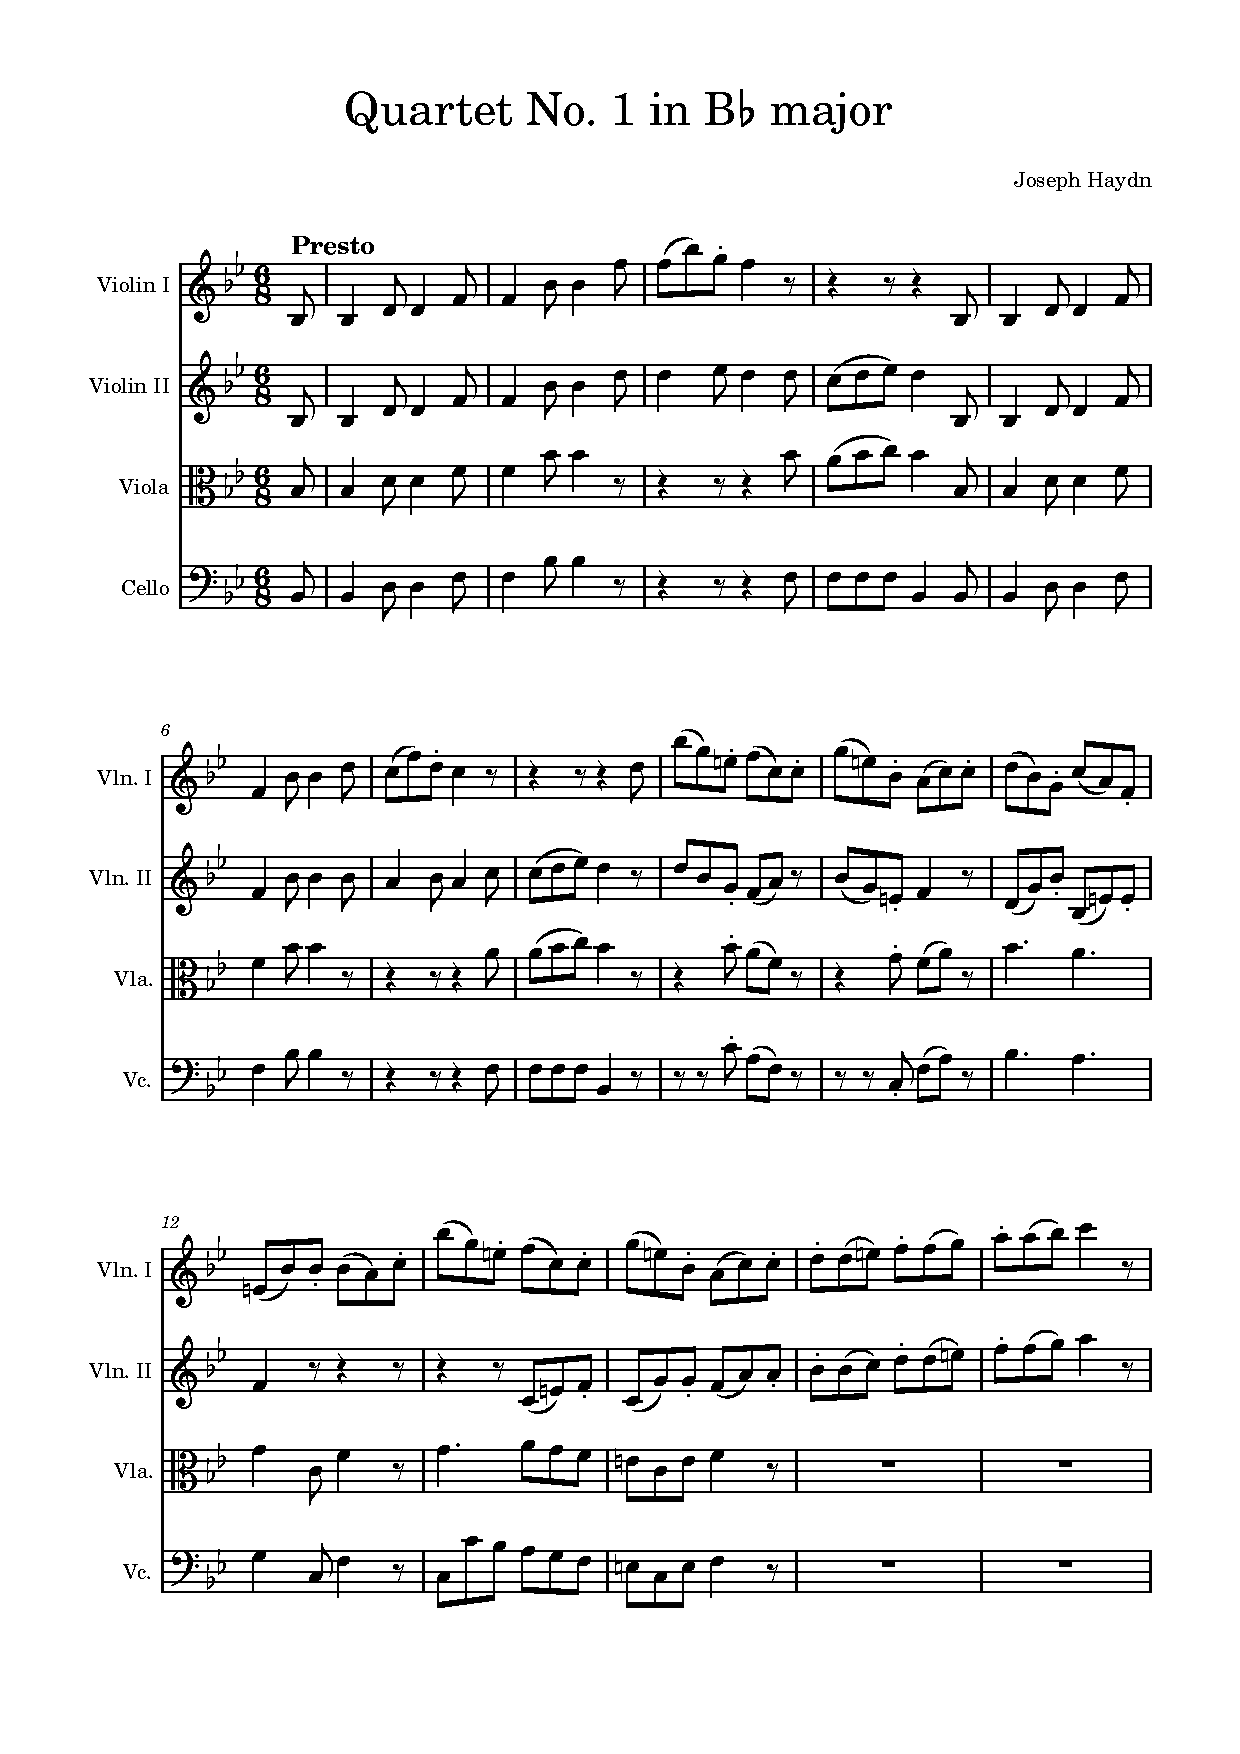
\includegraphics[width=\textwidth,page=1]{haydn-score.pdf}
    \caption{Quartet No.\ 1 in B-flat major, Op.\ 1, by Joseph Haydn, bars 1--16.}
    \label{fig:haydn-score}
\end{figure}

\begin{figure}
    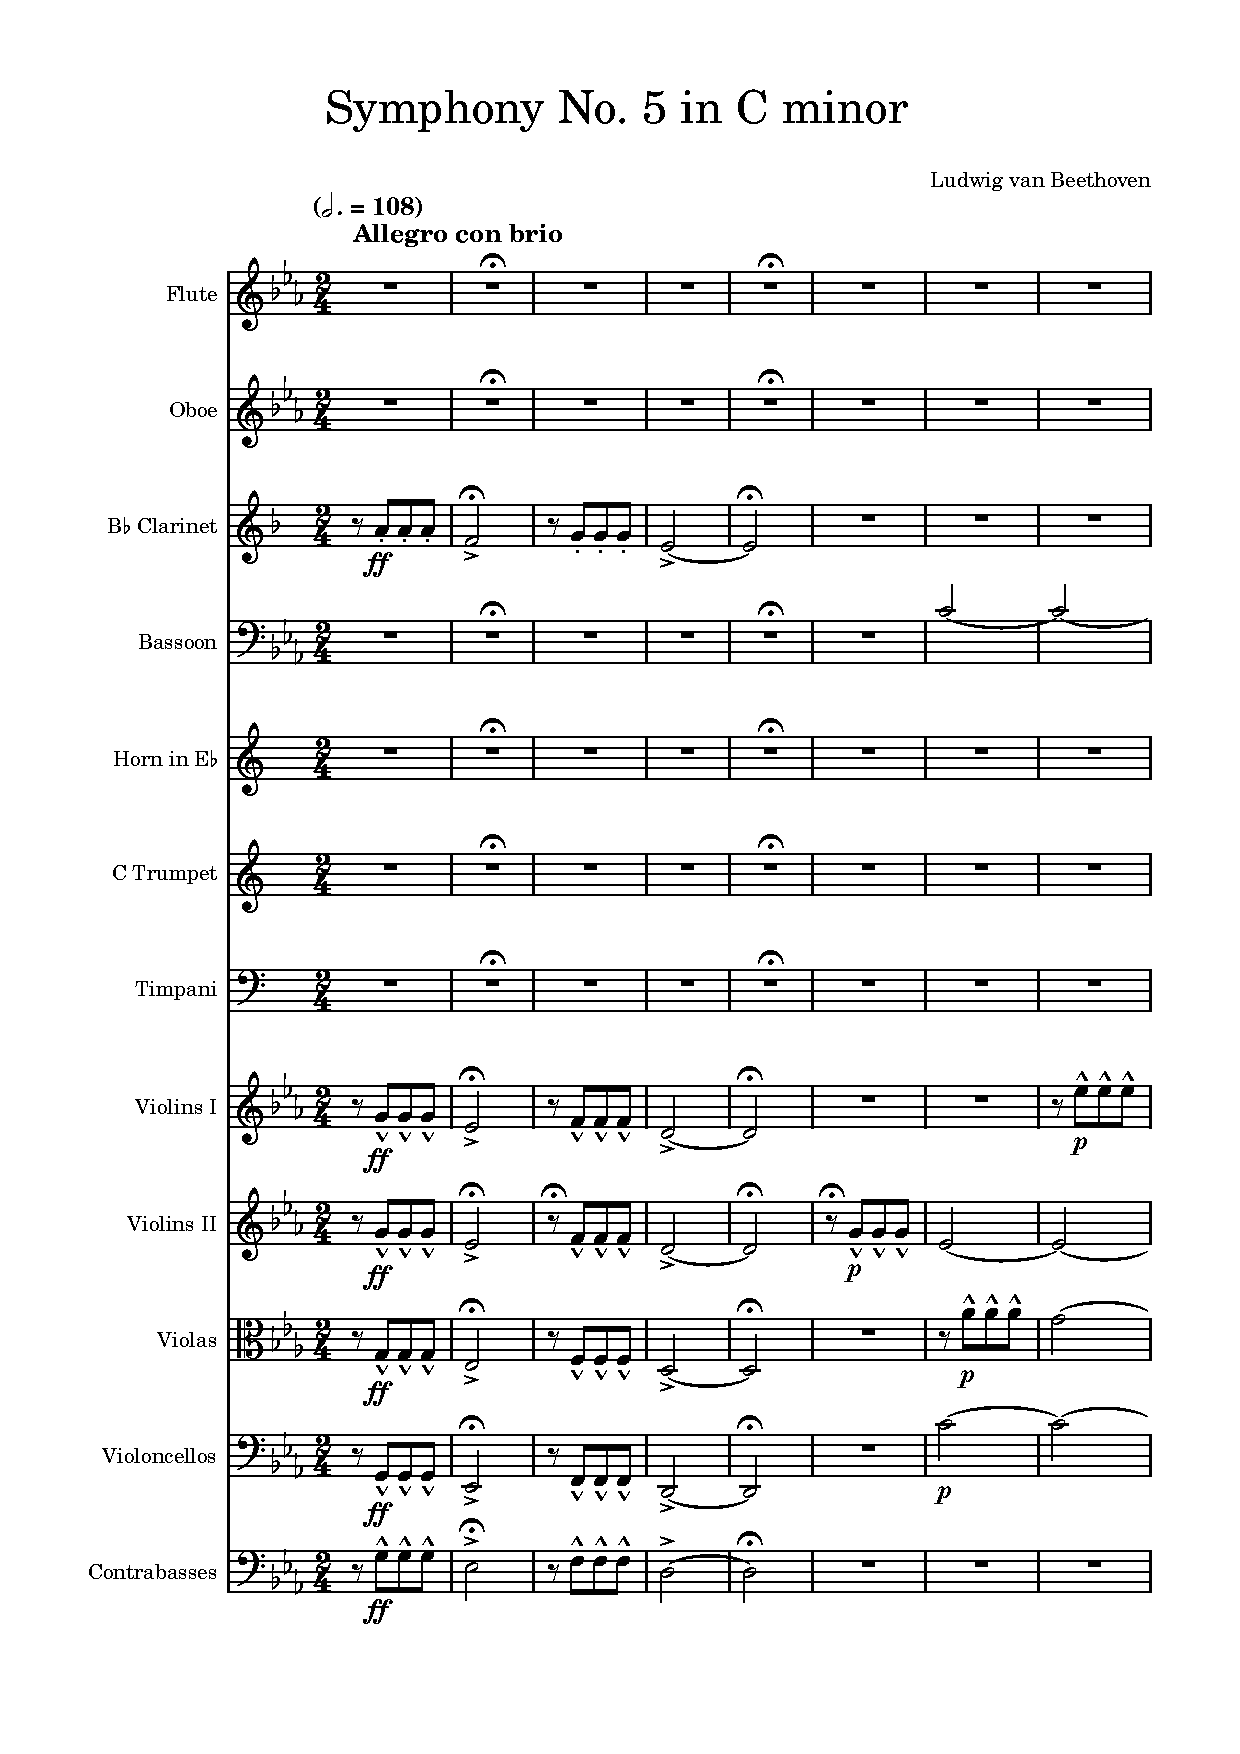
\includegraphics[width=\textwidth,page=1]{beethoven-op67.pdf}
    \caption{Symphony No.\ 5 in C minor, Op.\ 67, by Ludwig van Beethoven, bars 1--8.}
\end{figure}

\clearpage

\section*{Scientific summary for a general audience} % 200 words
\addcontentsline{toc}{section}{Scientific summary for a general audience}

The arrangement of music by hand is usually a difficult and time-consuming process, requiring a deep understanding of musical theory and structure. This study aims to automate this process via quantum computing, a technique that relies on the use of qubits, which can exist in a superposition of states. A music score can be split up into a sequence of phrases by looking at how much adjacent notes differ from each other, and turned into a graph representation with nodes and edges, where each node is a phrase, and edges between nodes mean they overlap. This graph can then be sent to a quantum computer in order to select nodes according to a set of rules that determine the properties of the arrangement. Once the nodes have been selected, the corresponding phrases can be reconstructed to create the final score. Here, an excerpt of Beethoven's String Quartet No.\ 10 is reduced to a single part, suitable for a solo instrument.

\end{document}